\documentclass[a4paper,12pt]{article}
\usepackage[utf8]{inputenc}
\usepackage{polski}
\usepackage{graphicx}
\usepackage{amsmath}
\usepackage{amssymb}
\usepackage{hyperref}
\usepackage{float}
\usepackage{listings}

\lstset{upquote=true}

\title{Sprawozdanie z laboratorium Hurtownie Danych}
\author{Mikołaj Kubś, 272662}
\date{\today}

\begin{document}

\maketitle

\section{Zadanie 1}
Analiza konceptualnego modelu danych "Usługi", który jest niekompletny,
ale klasy i relacje między nimi reprezentują rozpatrywany wycinek rzeczywistości. 

\begin{figure}[H]
\centering
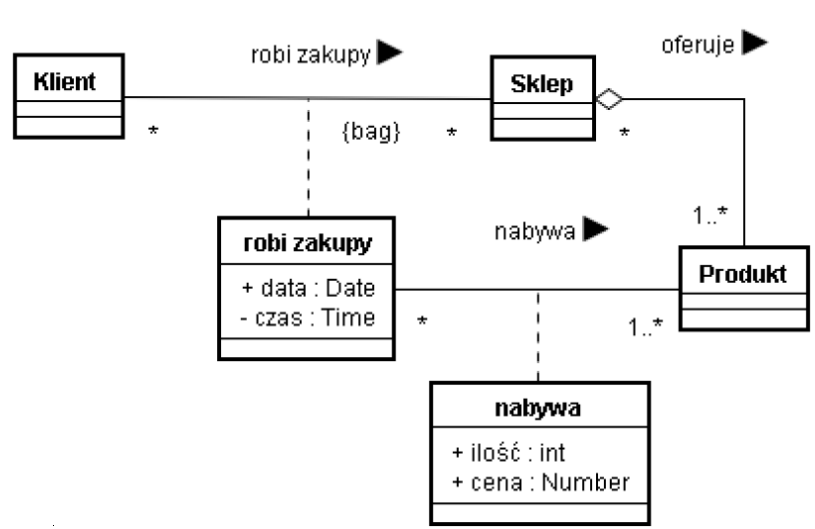
\includegraphics[width=0.8\textwidth]{images/old.png}
\caption{Konceptualny model danych "Usługi"}
\label{fig:uslugi}
\end{figure}

Reguły i ograniczenia dziedzinowe:
\begin{itemize}
    \item Reg/01 - Klient może wielokrotnie robić zakupy w tym samym sklepie
    \item Reg/02 - W sklepie może robić zakupy dowolny klient
    \item Reg/03 - Każdy zakup realizowany jest przez klienta w sklepie w określonym dniu i godzinie
    \item Reg/04 - Sklep musi oferować co najmniej jeden produkt
    \item Reg/05 - \ldots
\end{itemize}

\subsection{Weryfikacja i poprawa modelu danych}

Ponieważ reguły są niekompletne i nie w pełni poprawne, zdecydowałem się wprowadzić szereg zmian. 

Uznałem, że reguła "Reg/04 - Sklep musi oferować co najmniej jeden produkt" wprowadza niepotrzebną komplikację. Na przykład, według tej zasady, gdy sklep sprzedałby cały swój inwentarz, nie mógłby dalej istnieć w bazie danych.

Brakuje aktualnie informacji, jaka jest liczba dostępnego produktu w danym sklepie. Można wyciągnąć tą daną do nowej tabeli asocjacyjnej, do której można by dodatkowo dodać cenę produktu dla konkretnego sklepu, co zwiększa elastyczność na przyszłość i jest szeroko stosowaną praktyką w rzeczywistych sklepach. Tak więc sklep może oferować wiele produktów, każdy z własną cenę i ilością. 
Ponieważ tabela asocjacyjna "oferuje" ma cenę, można by usunąć cenę z tabeli asocjacyjnej "nabywa". Uznałem jednak, że ją zostawię, ponieważ cena oferty może się zmienić po zakupie produktu przez klienta. 
Sklepy mają często informację, że coś sprzedają, nawet jeśli nie ma tego chwilowo w magazynie, tak więc ustaliłem, że ilość oferowanego produktu to co najmniej 0, a nie koniecznie więcej niż zero, co wymuszałoby usunięcie oferty w przypadku braków w magazynie.

Można dodać parę atrybutów do encji. Do klienta dodam imię i nazwisko, a do produktu i do sklepu nazwę.

Warto również dodać standardowe ograniczenia wobec atrybutów encji. Zdecydowałem, że cena nie może być mniejsza od 0, ale może się mu równać - czasem są zaskakujące promocje w sklepach. Dodatkowo uznałem, że każdy produkt ma unikalną nazwę.

Oprócz tego dodałem reguły wynikające z diagramu klas, klaryfikujące, że:

\begin{enumerate}
    \item Klient może robić zakupy w różnych sklepach
    \item Ten sam produkt może być oferowany w wielu sklepach
    \item Klient robiący zakupy musi zakupić przynajmniej 1 produkt
\end{enumerate}

Dodatkowo zmieniłem typ atrybutów dotyczących kosztu na "decimal", a także zmieniłem atrybut "data" w "robi zakupy" na prywatny.

\newpage
\subsection{Finalna postać reguł, ograniczeń i diagramu klas UML}

Finalna postać reguł i ograniczeń:

\begin{itemize}
    \item Reg/01 - Klient może wielokrotnie robić zakupy w tym samym sklepie
    \item Reg/02 - W sklepie może robić zakupy dowolny klient
    \item Reg/03 - Każdy zakup realizowany jest przez klienta w sklepie w określonym dniu i godzinie
    \item Reg/04 - Każdy sklep ustala własną cenę oraz ilość oferowanego produktu 
    \item Reg/05 - Klient nabywając produkt w danym sklepie kupuje go za cenę oferowaną w sklepie, która zostaje zapamiętana
    \item Reg/06 - Sklep może zmienić cenę oferowanego produktu, co wpływa tylko na przyszłe zakupy
    \item Reg/07 - Klient może robić zakupy w różnych sklepach
    \item Reg/08 - Ten sam produkt może być oferowany w wielu sklepach
    \item Reg/09 - Klient robiąc zakupy musi nabyć co najmniej 1 produkt
    \item Reg/10 - Imię klienta nie może być puste
    \item Reg/11 - Nazwisko klienta nie może być puste
    \item Reg/12 - Ilosc oferowanego produktu nie może być mniejsza od zera
    \item Reg/13 - Cena oferowanego produktu nie może być mniejsza od zera
    \item Reg/14 - Ilość nabytego produktu musi być większa od zera
    \item Reg/15 - Cena nabytego produktu nie może być mniejsza od zera
    \item Reg/16 - Nazwa produktu nie może się powtarzać
\end{itemize}

\begin{figure}[H]
\centering
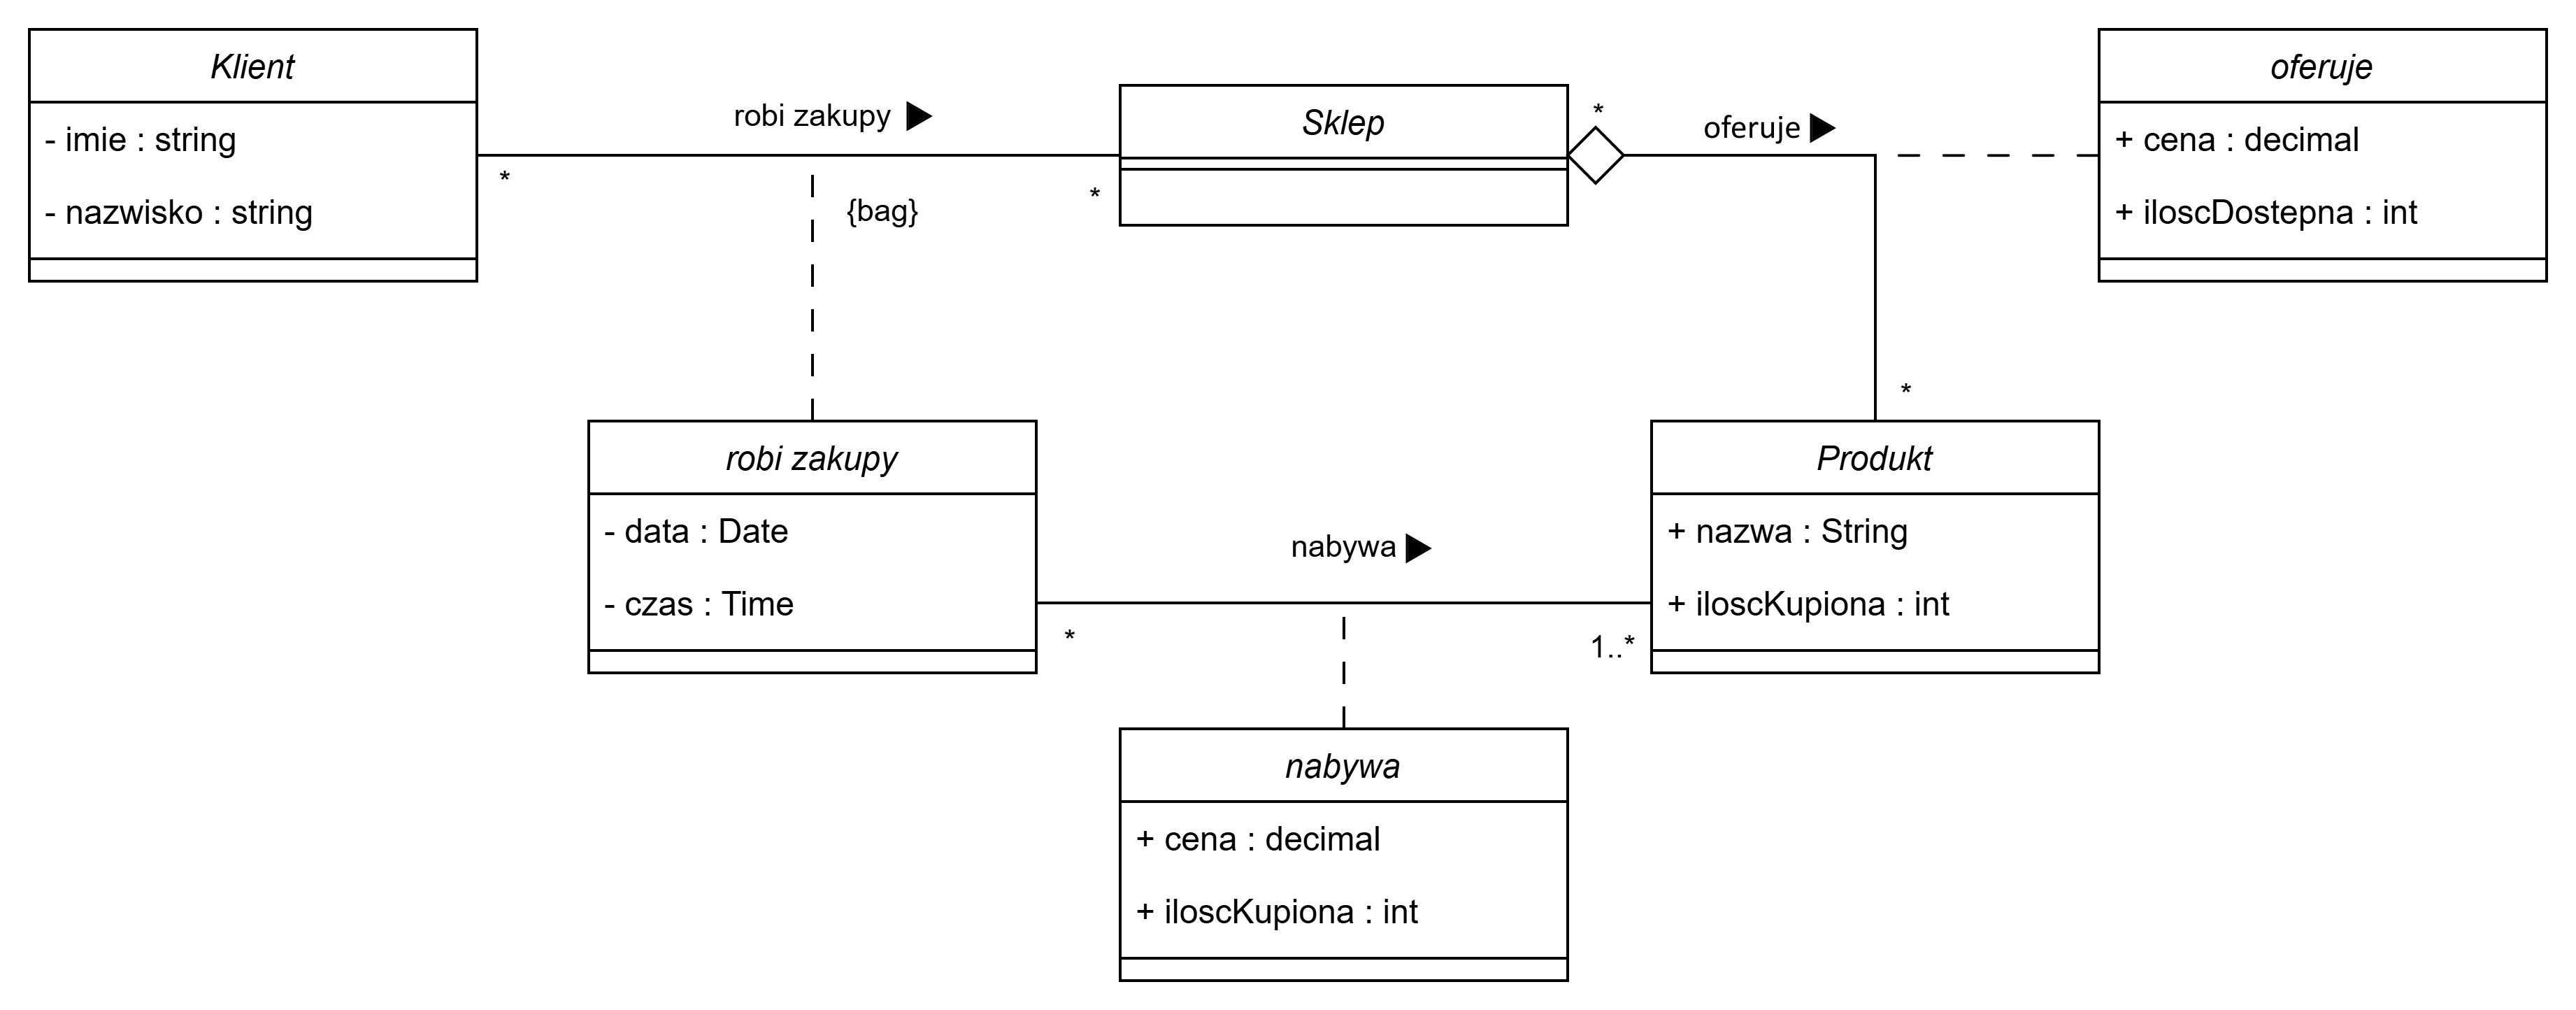
\includegraphics[width=0.8\textwidth]{images/improved.png}
\caption{Finalny model danych "Usługi"}
\label{fig:final_model}
\end{figure}

\subsection{Skrypt DDL SQL}

\begin{lstlisting}[
    language=SQL,
    showspaces=false,
    basicstyle=\ttfamily,
    numbers=left,
    numberstyle=\tiny,
    commentstyle=\color{gray}
 ]

 CREATE DATABASE Uslugi;
 GO
 
 USE Uslugi;
 
 DROP TABLE IF EXISTS Nabycie;
 DROP TABLE IF EXISTS Zakup;
 DROP TABLE IF EXISTS Oferta;
 DROP TABLE IF EXISTS Produkt;
 DROP TABLE IF EXISTS Sklep;
 DROP TABLE IF EXISTS Klient;
 
 CREATE TABLE Klient (
     id INT PRIMARY KEY,
     imie VARCHAR(255) NOT NULL,
     nazwisko VARCHAR(255) NOT NULL
 );
 
 CREATE TABLE Sklep (
     id INT PRIMARY KEY,
     nazwa VARCHAR(255) NOT NULL
 );
 
 CREATE TABLE Produkt (
     id INT PRIMARY KEY,
     nazwa VARCHAR(255) NOT NULL UNIQUE
 );
 
 CREATE TABLE Oferta (
     id INT PRIMARY KEY,
     cena DECIMAL(10,2) NOT NULL CHECK (cena >= 0),
     ilosc_dostepna INT NOT NULL CHECK (ilosc_dostepna >= 0),
     sklep_id INT NOT NULL,
     produkt_id INT NOT NULL,
     FOREIGN KEY (sklep_id) REFERENCES Sklep(id) ON DELETE CASCADE,
     FOREIGN KEY (produkt_id) REFERENCES Produkt(id) ON DELETE CASCADE
 );
 
 CREATE TABLE Zakup (
     id INT PRIMARY KEY,
     data DATE NOT NULL,
     czas TIME NOT NULL,
     klient_id INT,
     sklep_id INT NOT NULL,
     FOREIGN KEY (klient_id) REFERENCES Klient(id) ON DELETE SET NULL,
     FOREIGN KEY (sklep_id) REFERENCES Sklep(id) ON DELETE CASCADE,
     CONSTRAINT unique_zakup UNIQUE (data, czas, klient_id, sklep_id)
 );
 
 CREATE TABLE Nabycie (
     id INT PRIMARY KEY,
     cena DECIMAL(10,2) NOT NULL CHECK (cena >= 0),
     ilosc_kupiona INT NOT NULL CHECK (ilosc_kupiona > 0),
     zakup_id INT,
     oferta_id INT,
     FOREIGN KEY (zakup_id) REFERENCES Zakup(id) ON DELETE SET NULL,
     FOREIGN KEY (oferta_id) REFERENCES Oferta(id)
 ); 

\end{lstlisting}

\subsection{Inicjalizacja bazy danych w systemie MS SQL}

\subsection{Testy działania bazy danych}

\begin{figure}[H]
    \centering
    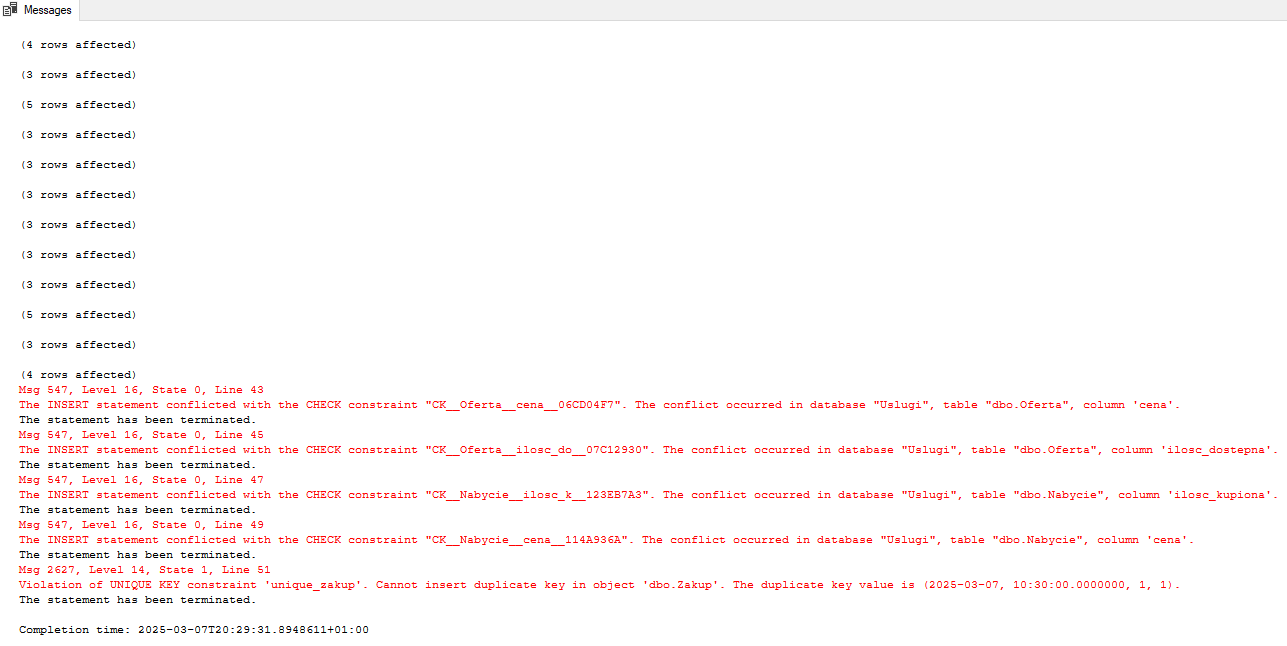
\includegraphics[width=0.8\textwidth]{images/seeding_console.png}
    \caption{Widok konsoli po wykonaniu poniższego kodu}
    \label{fig:tests}
    \end{figure}

INSERT INTO Klient (id, imie, nazwisko) VALUES
(1, 'Jan', 'Kowalski'),
(2, 'Anna', 'Nowak'),
(3, 'Piotr', 'Wójcik');

INSERT INTO Sklep (id, nazwa) VALUES
(1, 'Biedronka'),
(2, 'Biedronka'),
(3, 'BIEDRONKA pl. GRUNWALDZKI');

INSERT INTO Produkt (id, nazwa) VALUES
(1, 'Masło'),
(2, 'Bułki'),
(3, 'Wędliny');

INSERT INTO Oferta (id, cena, ilosc_dostepna, sklep_id, produkt_id) VALUES
(1, 25.99, 10, 1, 1),
(2, 45.50, 5, 1, 2),
(3, 15.75, 15, 2, 1),
(4, 35.30, 7, 2, 3),
(5, 99.99, 0, 3, 2);

INSERT INTO Zakup (id, data, czas, klient_id, sklep_id) VALUES
(1, '2025-03-07', '10:30:00', 1, 1),
(2, '2025-03-07', '11:00:00', 2, 2),
(3, '2025-03-07', '12:00:00', 3, 3);

INSERT INTO Nabycie (id, cena, ilosc_kupiona, zakup_id, oferta_id) VALUES
(1, 25.99, 3, 1, 1),
(2, 45.50, 2, 2, 2),
(3, 15.75, 5, 3, 3),
(4, 35.30, 1, 3, 4);

-- Invalid operations

INSERT INTO Oferta (id, cena, ilosc_dostepna, sklep_id, produkt_id) VALUES (6, -10.00, 10, 1, 1);

INSERT INTO Oferta (id, cena, ilosc_dostepna, sklep_id, produkt_id) VALUES (7, 20.00, -5, 1, 2);

INSERT INTO Nabycie (id, cena, ilosc_kupiona, zakup_id, oferta_id) VALUES (5, 25.00, 0, 1, 1);

INSERT INTO Nabycie (id, cena, ilosc_kupiona, zakup_id, oferta_id) VALUES (5, -25.00, 1, 1, 1);

INSERT INTO Zakup (id, data, czas, klient_id, sklep_id) VALUES (4, '2025-03-07', '10:30:00', 1, 1);

Wszystkie operacje zadziałały, oprócz tych, które naruszały ograniczenia.

\section{Zadanie 2}
Tutaj znajduje się cel laboratorium.

\begin{thebibliography}{9}
\bibitem{przyklad}
Autor, \textit{Tytuł}, Wydawnictwo, Rok.
\end{thebibliography}

\end{document}